\chapter{Sistemas de apoio à mulher em situação de violência} \label{cap:sistemas_relacionados}

Em uma geração dirigida pela tecnologia e engajamento em causas sociais é possível perceber que várias aplicações têm sido criadas em todo o mundo 
com o objetivo de apoiar a mulher vítima de violência. Com o intuito de entender o objetivo dessas aplicações e as lacunas que elas possuem,
foi realizado um levantamento das principais plataformas criadas. 

\section{Plataformas e aplicativos}

As plataformas identificadas foram: o site Minha Voz \cite{minhavoz_site} e 
os aplicativos Clique180, SalveMaria, SOSMulher e Lei Maria da Penha. Outros aplicativos e sites foram criados pela própria população, como: Juntas, Vazow, 
Chega de Fiufiu, 
SaiPraLá, PLP 2.0, Assédio Zero e Mete a Colher. Todas essas aplicações tratam de cenários comuns nas situações de 
violência.


\subsection*{Minha Voz}

Site criado no \textit{Hackathon} de Gênero e Cidadania, no qual
um dos temas era "Violência Contra a Mulher". 

De acordo com a documentação do site (disponível no GitHub \cite{minhavoz_repo}), o objetivo é ter um fórum para apoio às mulheres, no qual elas podem
realizar desabafos e obter um panorama da violência contra a mulher através de um questionário
disponível no site, relacionando os dados por:

\begin{itemize}
	\item Categorias;
	\item Locais;
	\item Grau de Proximidade com o agressor;
	\item Tempo de duração da violência;
	\item Data.
\end{itemize}

O site também disponibiliza um questionário para que a mulher possa identificar a categoria (tipo) da violência sofrida, respondendo a perguntas pré-definidas 
com "Sim" ou "Não". Esse questionário é construído baseado em uma árvore de decisão.

\vfill

\subsection*{Clique180}
Trata-se de um aplicativo criado pelo Onu Mulheres que, de acordo com
a página de download \cite{clique_180}, oferece:

\begin{itemize}
	\item Leis e conceitos;
	\item Localização e rotas até os serviços da rede de atendimento às mulheres;
	\item Botão para ligação para o 180;
	\item Dicas de ações a serem tomadas e tipos de serviços a procurar; 
	\item Mapeamento de locais de risco.
\end{itemize}

\subsection*{Salve Maria!}
Criado pelo governo do estado do Piauí, o SalveMaria \cite{salvemaria} é um aplicativo para envio de denúncias
de forma sigilosa, informando o tipo de assédio sofrido.
Além disso, conta com um Botão do Pânico que envia um pedido de socorro automaticamente para a polícia.

\subsection*{SOSMulher}
Aplicativo criado pelo governo do estado do Pará para mulheres que estão sob medida protetiva. 
De acordo com notícia publicada \cite{sosmulher}, 
o aplicativo é instalado no \textit{smartphone} e, quando a mulher está em situação de risco, por meio de três toques no aparelho, são enviadas notificações para a Central da Guarda Municipal.

\subsection*{Lei Maria da Penha}
Criado pelo programa interagencial de promoção da igualdade de gênero, raça e etnia, trata-se de um
aplicativo que contém toda a Lei Maria da Penha \cite{leimariadapenha}.

\subsection*{Juntas}
O site Juntas é um blog que contém \textit{posts} informativos, conceituais e notícias 
relacionadas ao cenário feminino no Brasil \cite{juntas}.

\subsection*{Vazow}

Aplicativo para vítimas de ``vingança pornô'', do inglês ``revenge porn'', que é a 
divulgação de vídeos e/ou fotos íntimas após término.
De acordo com a página de download \cite{vazow}, as funcionalidades oferecidas são:

\begin{itemize}
	\item Procedimentos e orientações para exclusão de conteúdo íntimo divulgado;
	\item Dicas de como evitar se tornar uma vítima;
	\item Legislação relacionada;
	\item Suporte para contato.
\end{itemize}

\subsection*{Chega de Fiufiu}

Um site no qual a mulher pode realizar uma denúncia de uma violência sofrida ou presenciada. 
Essa denúncia é realizada informando o endereço, o tipo de violência sofrida, a data, período do dia e o que foi feito. 
De acordo com o site \cite{chegadefiufiu}, o objetivo é ``mapear 
os lugares mais incômodos e até perigosos para mulheres no Brasil''.

\subsection*{SaiPraLá}

Aplicativo para realização de uma denúncia de violência informando o endereço em que o assédio ocorreu, 
o período do dia, o tipo de assédio e o que foi feito. 
De acordo com a página de download \cite{saiprala}, o objetivo é ``mapear o assédio e atuar na prevenção dele''.

\subsection*{PLP 2.0}
Aplicativo que possui um detector de emergência para acionar diretamente as redes de atendimento 
e também realiza a gravação de áudios e vídeos \cite{plp}.

\subsection*{Assédio Zero}

Aplicativo para as mulheres denunciarem dois tipos de agressão: física ou verbal, marcando a localização 
onde a violência ocorreu. Assim como os outros aplicativos de denúncia, o Assédio Zero \cite{assediozero}
tem como objetivo mapear a violência contra a mulher.

% \section{Apoio contextualizado}

% Em suma, as aplicações auxiliam nas denúncias, gerando dados como locais de riscos e estatísticas e
% apresentam informações genéricas sobre como agir em situações de violência. Dessa forma, percebe-se uma lacuna em um apoio contextualizado de acordo com a situação de violência vivida pela mulher.

% Um projeto australiano, chamado I-DECIDE, trata da violência doméstica disponibilizando um site para mulheres avaliarem sua relação, suas prioridades e planejar um futuro mais seguro através de um questionário. A ferramenta compreende avaliações de segurança e um processo de planejamento de ação individualizado adaptado às circunstâncias particulares de cada mulher \cite{idecide}.

\section{Comparativo entre as plaformas e aplicativos}

Considerando as informações de cada sistema, foi possível perceber que as aplicações têm funcionalidades
em comum e assim estabelecer cinco categorias de funcionalidades: Levantamento de Dados e estatísticas, Mapeamento de riscos, 
Informativos , Pedido de Socorro e Denúncia. Na Figura \ref{fig:sistemas_categorizados} é apresentado o mapeamento das aplicações com as categorias criadas e na 
Tabela \ref{tab:principais_funcionalidades} são apresentadas as principais funcionalidades em comum encontradas nos sistemas, 
de acordo com essas categorias.

\begin{figure}[h!]
\centering
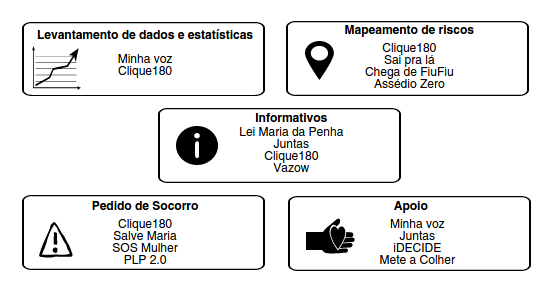
\includegraphics[scale=0.75]{figuras/sistemas_relacionados.png}
\caption{Aplicações de apoio à mulher vítima de violência}
\label{fig:sistemas_categorizados}
\end{figure}

Na categoria de Levantamento de Dados e estatísticas foram mapeadas as aplicações que possuem
o intuito de obter dados estatísticos sobre a violência de acordo com as respostas/denúncias das mulheres.

A categoria de Mapeamento de riscos também trata das aplicações que obtém os dados de violência através
das respostas/denúncias das mulheres, porém com o objetivo de mostrá-las os locais de risco.

As aplicações com finalidade de pedido de socorro automático foram categorizadas em Pedido de Socorro. 
E por fim, na categoria de Denúncia estão as aplicações que tem funcionalidade para realização de denúncias de violência
para autoridades competentes ou como uma forma de compartilhar o que aconteceu.

\begin{table}[h]
\centering
\caption{Funcionalidades encontradas nos sistemas relacionados}
\label{tab:principais_funcionalidades}
\begin{tabular}{l|l}
\hline
\multicolumn{1}{c|}{\textbf{Categoria}} & \multicolumn{1}{c}{\textbf{Funcionalidades}} \\ \hline
\begin{tabular}[c]{@{}l@{}} Levantamento de Dados\\ e estatísticas\end{tabular} & \begin{tabular}[c]{@{}l@{}} - Categorização e junção dos dados obtidos de cada mulher \\ (através de questionário ou formulário de denúncia)\end{tabular} \\ \hline 
Mapeamento de Riscos & \begin{tabular}[c]{@{}l@{}}-  Mapeamento de locais de riscos por meio das denúncias de \\ violência realizadas\end{tabular} \\ \hline
Informativos & \begin{tabular}[c]{@{}l@{}} - Disponibilização de leis e conceitos relacionados \\ - Auxílio na descoberta da violência sofrida \\ - Disponibilização de notícias\end{tabular}  \\ \hline
Pedidos de Socorro & - Envio de pedido de socorro às autoridades competentes \\ \hline
Denúncia & \begin{tabular}[c]{@{}l@{}}- Denúncia da violência sofrida às autoridades competentes\\ - Compartilhamento da
violência sofrida para: \\ \hspace{1em} - alerta à outras mulheres \\ \hspace{1em} - levantamento de dados \end{tabular} \\ \hline
\end{tabular}
\end{table}


Em suma, as aplicações auxiliam nas denúncias, gerando dados como locais de riscos e estatísticas e
apresentam informações genéricas sobre como agir em situações de violência. 
Contudo, percebe-se uma lacuna, pois há dispersão dos dados, estatísticas e mapeamentos realizados em cada aplicação.

Além disso, as discussões encontradas nas plataformas são restritas à notícias e desabafos e nota-se a falta de um espaço
para debates e discussões mais efetivas acerca do assunto, ou seja, discussões que gerem resultados para a sociedade
como um todo, principalmente no que se refere a criação de políticas públicas.

A ideia da plataforma ``Empurrando Juntos'' de expor todos os pensamentos e poder promover uma discussão sobre um 
determinado
assunto configura uma outra abordagem na tentativa de mitigar essa lacuna identificada.

